\documentclass[a4paper,11pt]{article}
	%INCLUDE DEL TEMPLATE
		\usepackage[utf8]{inputenc}
	\usepackage[italian]{babel}
	\usepackage{hyperref}	%Consente l'inserimento di \url
	\usepackage{booktabs}	%Utilità di abbellimento tabelle
	\usepackage{longtable}
	\usepackage{tabularx}
	%\usepackage{widetable}
	\usepackage{array}
	\usepackage{listings}
	\usepackage{graphicx}
	\usepackage{caption}
	\usepackage{fancyhdr}
	\newenvironment{fixpic}{}{} % [1]
	\usepackage[a4paper,top=3cm,bottom=3cm,left=2.5cm,right=2.5cm]{geometry}
	%******
	\usepackage{makeidx}
	\usepackage{textcomp}
	\usepackage{multirow}
	\usepackage{rotfloat}
	\usepackage{lastpage}
	\usepackage{array}
	\usepackage{float}
	% *************************************
	% QUI CODICE PER \SUBSUBSUBSECTION
	\usepackage{titlesec}
	\titleclass{\subsubsubsection}{straight}[\subsection]
	
	\newcounter{subsubsubsection}[subsubsection]
	\renewcommand\thesubsubsubsection{\thesubsubsection.\arabic{subsubsubsection}}
	\renewcommand\theparagraph{\thesubsubsubsection.\arabic{paragraph}} % optional; useful if paragraphs are to be numbered
	
	\titleformat{\subsubsubsection}
	  {\normalfont\normalsize\bfseries}{\thesubsubsubsection}{1em}{}
	\titlespacing*{\subsubsubsection}
	{0pt}{3.25ex plus 1ex minus .2ex}{1.5ex plus .2ex}
	
	\makeatletter
	\renewcommand\paragraph{\@startsection{paragraph}{5}{\z@}%
	  {3.25ex \@plus1ex \@minus.2ex}%
	  {-1em}%
	  {\normalfont\normalsize\bfseries}}
	\renewcommand\subparagraph{\@startsection{subparagraph}{6}{\parindent}%
	  {3.25ex \@plus1ex \@minus .2ex}%
	  {-1em}%
	  {\normalfont\normalsize\bfseries}}
	\def\toclevel@subsubsubsection{4}
	\def\toclevel@paragraph{5}
	\def\toclevel@paragraph{6}
	\def\l@subsubsubsection{\@dottedtocline{4}{7em}{4em}}
	\def\l@paragraph{\@dottedtocline{5}{10em}{5em}}
	\def\l@subparagraph{\@dottedtocline{6}{14em}{6em}}
	\makeatother
	
	\setcounter{secnumdepth}{4}
	\setcounter{tocdepth}{4}
	%FINE \SUBSUBSUBSECTION
	%****************************************
	%STYLE PER INSERIMENTO DEL CODICE
	\lstdefinestyle{style1}{
	  belowcaptionskip=1\baselineskip,
	  breaklines=true,
	  frame=L,
	  xleftmargin=\parindent,
	  language=Pascal,
	  showstringspaces=false,
	  basicstyle=\footnotesize\ttfamily,
	  keywordstyle=\bfseries\color{blue},
	  commentstyle=\itshape\color{blue},
	  identifierstyle=\color{blue},
	  stringstyle=\color{orange},
	}
	
	\lstdefinestyle{style2}{
	  belowcaptionskip=1\baselineskip,
	  frame=L,
	  xleftmargin=\parindent,
	  language=C,
	  basicstyle=\footnotesize\ttfamily,
	  commentstyle=\itshape\color{blue},
	}
	\lstset{style=style1}
	
	%FINE STYLE INSERIMENTO CODICE
	%*****************************************
	\usepackage[default]{cantarell} %% Use option "defaultsans" to use cantarell as sans serif only
	\usepackage[T1]{fontenc}        %% for font
	\hypersetup{colorlinks, linkcolor=black, urlcolor=blue}
	\newcommand{\addglos}{\begin{scriptsize}{\textbf{\ped{G}}} \end{scriptsize}} 
	\pagestyle{fancy}
	\fancyhead{}
	\fancyfoot{}
	%\fancyhead[L]{
\includegraphics[scale=0.28]{team_not_found.jpeg}}
	\fancyhead[L]{
\includegraphics[scale=0.15]{../../team404_small.jpg} \hspace{2mm} QUIZZIPEDIA}
	\fancyhead[R]{\leftmark}
	\fancyfoot[L]{Universit\`a degli studi di Padova - IS 2015/2016 \\ \url{team404swe@gmail.com}}

	
	%Commando usato per la tabella di informazioni sul documento
	\newcommand{\introtab}[9]{
		\begin{table}[ht]
		\begin{center}		
		\begin{tabular}{r l}			
			\toprule		
			\multicolumn{2}{c}{\textbf{ Informazioni sul documento }} \\
			\midrule 
			\textbf{Nome Documento}			& \vline \hspace{3.5 mm} {#1} \\
			\textbf{Versione}				& \vline \hspace{3.5 mm} {#2} \\
			\textbf{Uso} 					& \vline \hspace{3.5 mm} {#3} \\
			\textbf{Data Creazione} 		& \vline \hspace{3.5 mm} {#4} \\
			\textbf{Data Ultima Modifica} 	& \vline \hspace{3.5 mm} {#5} \\
			\textbf{Redazione}				& \vline \hspace{3.5 mm} {#6} \\
											%& \vline \hspace{3.5 mm} {#7} \\	
			\textbf{Verifica} 				& \vline \hspace{3.5 mm} {#7}	\\
			\textbf{Approvazione}			& \vline \hspace{3.5 mm} {#8}\\	
			\textbf{Committente} 			& \vline \hspace{3.5 mm} Zucchetti SPA\\
			\textbf{Lista di distribuzione} & \vline \hspace{3.5 mm} Prof. Vardanega Tullio \\														& \vline \hspace{3.5 mm} TEAM404 \\
	\bottomrule	
	\end{tabular}
	\end{center}
	\end{table}
	}
	% Comando di inizio del registro
	\newcommand{\beginregistro}{
		%\begin{longtable}{{|p{0.10\textwidth}|p{0.20\textwidth}|p{0.15\textwidth}|p{0.50\textwidth}|}}
		\begin{longtable}{{|p{1.5cm}|p{2.5cm}|p{2cm}|p{8cm}|}} 
	 		\hline	
	}
	% commando usato pr inserire una riga al registro delle modifiche
	\newcommand{\rigaregistro}[4]{
		{\footnotesize #1} & {\footnotesize #2} &  {\footnotesize #3} &  {\footnotesize #4} \\
			\hline	
	}
	% Comando di fine registro
	\newcommand{\fineregistro}{ \end{longtable}	}
	
	%************************************************
	% commandi per il GLOSSARIO
	%***********************************************
	% Commando di inizio tabella Glossario
	\newcommand{\beginglos}{
		\begin{longtable}{{p{0.20\textwidth}p{0.65\textwidth}}}	
	}
	% Commando per i termini del glossario
	
	\newcommand{\itemglos}[2]{
		\textbf{#1 :} & {#2} \\ \\ \\
	}
	% Commando fine Glossario
	\newcommand{\fineglos}{ \end{longtable} }
	% Comando per aggiungere una ssezione numerata con lettere al glossario
	\newcommand{\sezione}{
	\subsection{}	
	\rule[0.3pt]{\linewidth}{0.4pt} \\ % Linea orizzontale
	}
	
\newcommand{\sezioneglos}[1] { 
  \newpage
  \cleardoublepage
  \phantomsection
  \addcontentsline{toc}{section}{#1}
  \vspace{11pt}
  \textbf{\huge{#1} } % Lettera grande 
  \\
  \rule[0.3pt]{\linewidth}{0.4pt} \\ % Linea orizzontale
  \fancyhead[R]{#1}
}

	\title{\textbf{{\fontsize{8mm}{5mm}\selectfont QUIZZIPEDIA}}}
	\date{}
	\author{}	


\begin{document}
	%\title{Piano di Qualifica} comment by Martin
	%\author{Andrea Multineddu}
	\maketitle
	% da qui : add by Martin
	\thispagestyle{empty}
	\begin{center}	
	
\includegraphics{../../team_not_found}\\
	\fontsize{5mm}{3mm}\url{team404swe@gmail.com}\\
	
	\vspace{50mm}
	\textbf{Piano di qualifica 1.0}
	%\'end{center}
	%\'begin{center}
	%\vspace{4mm}
	\end{center}
	\introtab{Piano di qualifica}			%1 nome documento
			{1.0} 							%2 versione
			{Esterno} 						%3 Uso
			{21 dicembre 2015} 				%4 Data cre
			{\today} 						%5 Data mod
			{Andrea Multineddu}	%6 Redazione
			{Marco Crivellaro - Luca Alessio } 			%7 Verifica
			{Davide Bortot } 				%8 Approvazione
	%fino a qui : add by Martin
	\newpage
	\thispagestyle{empty}
	\null  % add by Martin

	%\null	comment by Martin
	\newpage
	\newpage
	\fancyhead[R]{REGISTRO DELLE MODIFICHE}
	\fancyfoot[R]{\thepage}
	
	\hspace{30 mm}
	\section*{Registro delle modifiche}
	
	\beginregistro
	\rigaregistro{\textbf{Versione}}{\textbf{Autore}}{\textbf{Data}}		 {\hspace{5 mm} \textbf{Descrizione}}
	\rigaregistro{1.5}{A. Beccaro (Verificatore)}{27/04/2016}{Rivista sezione gestione amministrativa, aggiunta sezione procedure controllo qualità processi, rifatta sezione organizzazione}
	\rigaregistro{1.4}{A. Beccaro (Verificatore)}{26/04/2016}{rivista sezione verifica fasi di sviluppo}
	\rigaregistro{1.3}{A. Beccaro (Verificatore)}{25/04/2016}{Ampliato paragrafo sui parametri di tolleranza}
	\rigaregistro{1.2}{A. Beccaro (Verificatore)}{17/04/2016}{Aggiunto paragrafo "Procedure di controllo di qualità processi"}
	\rigaregistro{1.1}{A. Beccaro (Verificatore)}{16/04/2016}{Modifica struttura documento in seguito alla RR}
	\rigaregistro{1.0}{D. Bortot (Responsabile)}{16/03/2016}{Approvazione documento.}
	\rigaregistro{0.2}{L. Alessio (Verificatore)}{15/03/2016}{Verifica documento completo.}
    	\rigaregistro{0.1.1}{A. Multineddu (Verificatore)}{11/03/2016}{Correzione errori di impaginazione e tipografici}	
	\rigaregistro{0.1}{M. Crivellaro (Verificatore)}{10/03/2016}{Verifica documento.}
	\rigaregistro{0.0.7}{A. Multineddu (Verificatore)}{19/01/2016}{Correzione errori nella sezione Misure e metriche}
	\rigaregistro{0.0.6}{A. Multineddu (Verificatore)}{18/01/2016}{Aggiunta metriche e tabella resoconto misure}
	\rigaregistro{0.0.5}{M. Crivellaro (Verificatore)}{16/01/2016}{Modifica layout e aggiunta file template.tex}
	\rigaregistro{0.0.4}{A. Multineddu (Verificatore)}{07/01/2016}{Redazione sezione Misure e metriche}
	\rigaregistro{0.0.3}{A. Multineddu (Verificatore)}{03/01/2016}{Redazione sezione Risorse per la verifica}
\rigaregistro{0.0.2}{A. Multineddu (Verificatore)}{22/12/2015}{Redazione sezione Strategia generale di qualifica}			
		\rigaregistro{0.0.1}{A. Multineddu (Verificatore)}{21/12/2015}{Prima stesura del documento.}
			
	\fineregistro
	\newpage
	\fancyhead[R]{\leftmark} % add by Martin 
	\tableofcontents
	\pagenumbering{Roman}

	%\newpage %Comment by Martin
	\listoffigures	
	
	\newpage
	\pagenumbering{arabic}
	
	\section*{Sommario}
	Il presente documento contiene il \textit{piano di qualifica} del capitolato \textbf{Quizzipedia}. Vengono rese note le strategie di verifica qualitativa dei processi e del prodotto utilizzate dal gruppo \textbf{Team404}. Strategie che coinvolgono l'attuazione di modelli standard e l'utilizzo di metriche e misure necessarie alla valutazione oggettiva del processo o prodotto in analisi.  
	
	\newpage
	\section{Introduzione}
	\subsection{Scopo del documento}
	Questo documento ha lo scopo di esporre le strategie che il gruppo \textbf{Team404} intende adottare per assicurare la qualità del prodotto software \textbf{Quizzipedia} e dei processi coinvolti per il suo sviluppo.
	
	
	\subsection{Scopo del prodotto}
	Il progetto \textbf{Quizzipedia} ha come obiettivo lo sviluppo di un sistema software basato su tecnologie Web (Javascript\addglos, Node.js\addglos, HTML5\addglos, CSS3\addglos) che permetta la creazione, gestione e fruizione di questionari. Il sistema dovrà quindi poter archiviare i questionari suddivisi per argomento, le cui domande dovranno essere raccolte attraverso uno specifico linguaggio di markup (Quiz Markup Language) d'ora in poi denominato QML\addglos. In un caso d'uso a titolo esemplificativo, un "esaminatore" dovrà poter costruire il proprio questionario scegliendo tra le domande archiviate, ed il questionario così composto sarà presentato e fruibile all' "esaminando", traducendo l'oggetto QML in una pagina HTML\addglos, tramite un'apposita interfaccia web. Il sistema presentato dovrà inoltre poter proporre questionari preconfezionati e valutare le risposte fornite dall'utente finale.
	\\
	Per un'analisi più precisa ed approfondita del progetto si rimanda al documento\\ "\textit{analisi\_dei\_requisiti\_1.0.pdf}".
	\subsection{Glossario}
	Viene allegato un glossario nel file ``\textit{glossario\_1.0.pdf}'' nel quale viene data una definizione a tutti i termini che in questo documento appaiono con il simbolo '\addglos' a pedice.
	\newpage
	\subsection{Riferimenti}
		\subsubsection{Normativi}
		\begin{itemize}
			\item Capitolato d'appalto Quizzipedia:\\
			\url{http://www.math.unipd.it/~tullio/IS-1/2015/Progetto/C5.pdf}
			\item Norme di Progetto: "\textit{norme\_di\_progetto\_1.0.pdf}"
		\end{itemize}
		\subsubsection{Informativi}
		\begin{itemize}
			\item Corso di Ingegneria del Software anno 2015/2016:\\
			\url{http://www.math.unipd.it/~tullio/IS-1/2015/}
			\item Regole del progetto didattico:\\
			\url{http://www.math.unipd.it/~tullio/IS-1/2015/Dispense/PD01.pdf}
			\url{http://www.math.unipd.it/~tullio/IS-1/2015/Progetto/}\\
			\url{http://www.math.unipd.it/~tullio/IS-1/2015/Progetto/PD01b.html}
			\item Metriche di progetto:\\ 
			\url{https://it.wikipedia.org/wiki/Metriche_di_progetto}
			\item Metriche per il software\\
			\url{http://www.verifysoft.com/en_software_complexity_metrics.pdf}
			\item Complexity-report:\\
			\url{https://github.com/jared-stilwell/complexity-report}
		\end{itemize}
	\pagebreak
	
\newpage

\section{Strategia generale di qualifica}
\subsection{Definizione obiettivi}
Il gruppo di lavoro, per garantire la qualità del prodotto software \textbf{Quizzipedia} e dei processi coinvolti al suo sviluppo, intende adottare metodologie standard ed il più possibile automatizzabili per ridurre al minimo l'attività umana e favorire processi automatici laddove sia possibile.\\
Vengono di seguito quindi elencati gli obiettivi di qualità che si vogliono raggiungere per quanto riguarda il prodotto finale e i processi coinvolti per lo sviluppo dello stesso, e le strategie necessarie all'attuazione della corretta verifica e validazione del prodotto.\\
Lo scopo principale è quello di rendere definibili e misurabili tutti i processi di sviluppo e verifica per poterne controllare l'andamento e la produttività. 
\subsubsection{Qualità di processo}
Per quanto riguarda la valutazione qualitativa dei processi si fa riferimento a due modelli: 
\begin{itemize}
\item SPICE\addglos : definito dallo standard \underline{ISO/IEC 15504:1998}, fornisce un modello per la valutazione del livello di “maturità”
dei processi per identificare quali azioni possono essere necessarie per migliorare un processo specifico.
\item PDCA\addglos : metodo di gestione iterativo utilizzato per il controllo e il miglioramento continuo dei processi e dei prodotti. 
\end{itemize}

\textbf{DA DESCRIVERE IN APPENDICE I DUE MODELLI}
\subsubsection{Qualità di prodotto}
Come punto di riferimento per la qualità del prodotto software si fa riferimento allo standard \underline{ISO/IEC 9126:2001}.\\
L'immagine seguente elenca le principali caratteristiche a cui un prodotto software di qualità deve aspirare:\\
\begin{figure}[h!]
\centering
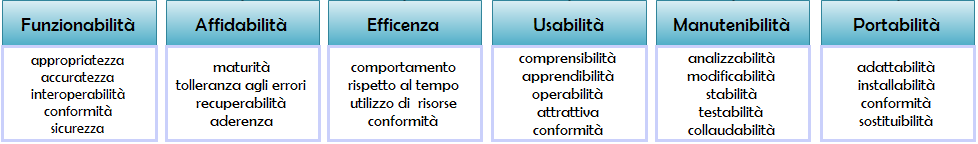
\includegraphics[scale=0.55]{../images/ISO-9126-cut}
\caption{Riepilogo caratteristiche ISO/IEC 9126:2001}
\end{figure}

\textbf{DA DESCRIVERE IN APPENDICE}
%\subsection{Pianificazione attività di sviluppo}
%La suddivisione temporale delle diverse fasi di sviluppo segue il cosiddetto modello a V ed è descritta nel documento allegato \textit{Piano-di-Progetto-1.0.pdf}.
%\begin{figure}[h!]
%\centering
%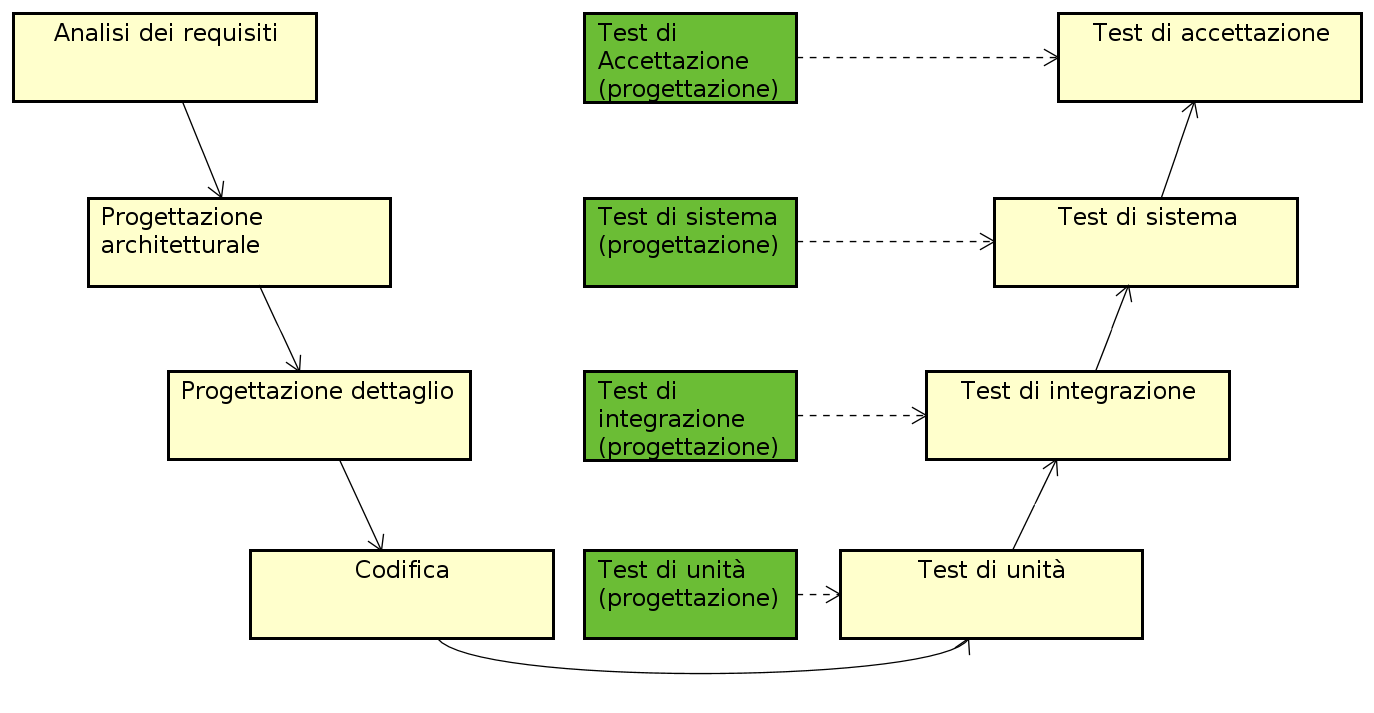
\includegraphics[scale=0.4]{../images/vmodel-final4.png}
%\caption{Fasi di sviluppo}
%\end{figure} 
%%questo paragrafo era abbastanza da rivedere, ora credo sia più chiaro ma aspetto anche la revisione di andrea e casomai lo modificheremo ancora
%Questo modello prevede un lavoro di controllo e verifica corrispondente ad ogni attività per evitare l'accumulo di errori difficilmente gestibili in seguito.\\
%La divisione in diverse fasi, e l'attività di verifica abbinata ad ogni fase e processo, hanno come scopo quello di facilitare l'integrazione e il corretto funzionamento delle parti che comporranno il sistema finale.
%Il ramo discendente descritto nella precedente figura rappresenta la successione delle fasi di sviluppo: ciascuna fase è accompagnata da una costante attività di verifica in modo da poter permettere il passaggio alla fase successiva esclusivamente quando si è sicuri che non ci siano errori. Ciò è essenziale durante la delicata attività di raccolta e documentazione dei requisiti, nella progettazione architetturale ad alto livello ed in seguito nella progettazione di dettaglio.\\ 
%%in questa frase non capivo proprio cosa volevi dire, nel dubbio sotto la mia frase ti lascio quello che avevi scritto se vuoi rimetterlo
%Del ramo ascendente che attraversa le attività di testing è importante sottolineare l'utilizzo dell'approccio bottom-up.
%%Per quanto riguarda il ramo ascendente, da notare l'essenziale importanza, per l'attività di testing,  dell'approccio bottom-up che inizia nel ramo più basso del diagramma. 
%Dalla fase di codifica quindi, per mezzo di test specifici sulle singole componenti (test di unità), si è in grado di garantire la correttezza del lavoro svolto prima che le singole componenti vengano integrate tra loro. Ovviamente l'esito positivo di ogni test su ogni unità non garantisce la correttezza dell'integrazione tra le stesse. \\
%Nelle sezioni successive verranno elencate le varie fasi del ramo discendente e ne verranno descritte le strategie di verifica qualitativa inerenti.
\newpage
\subsection{Organizzazione}
Di seguito vengono descritte le attività di verifica da effettuare per ogni fase di sviluppo. Tali fasi seguono la pianificazione definita nel documento allegato \textit{Piano-di-progetto-2.0.pdf}.
\subsubsection{Analisi}
\begin{itemize}
\item \textbf{Organizzazione interna}:
\begin{itemize}
\item \textbf{Assegnazione dei ruoli} secondo la pianificazione specificata nel documento \textit{Piano-di-Progetto-1.0.pdf} redatto dal Responsabile di progetto;
\item \textbf{Corretta pianificazione di sviluppo} secondo quanto stilato sempre nel documento \textit{Piano-di-Progetto-1.0.pdf}. In particolare viene verificata la corretta divisione temporale delle diverse fasi di progetto (vedere sezione precedente) e la correttezza del preventivo in base al budget disponibile;
\item \textbf{Disponibilità delle risorse umane e tecnologiche} e dell'ambiente di lavoro;
\item \textbf{Lettura e sottoscrizione delle Norme di Progetto}. Il responsabile deve accertarsi che ogni membro del gruppo abbia letto e compreso il documento \textit{Norme-di-progetto-1.0}. Il documento deve essere quindi preventivamente redatto.


\end{itemize} 
 
\item \textbf{Documentazione}: il processo di verifica per la documentazione deve seguire le linee guida descritte nella sezione 3 (Misure e metriche: parametri di tolleranza).
%\begin{itemize}
%\item Verifica della presenza di tutti i documenti necessari;
%\item Attinenza di ogni documento alle specifiche di stile e formattazione presenti nel documento \textit{Norme-di-progetto-1.0};
%\item Verifica della presenza e del corretto utilizzo del registro delle modifiche interno ad ogni documento;
%\item Verifica iniziale dei documenti tramite la tecnica di analisi statica \textbf{walkthrough};
%\item Verifica dei documenti tramite tecnica di analisi statica di tipo \textbf{inspection}. In questo caso l'attenzione del verificatore si focalizza solo su particolari aspetti del testo (per esempio accenti, sillabazione, maiuscole, ecc);
%\item Monitoraggio da parte dei verificatori del registro delle modifiche in modo da poter attuare la verifica solo alla parte inerente alla sezione modificata;
%\item \textbf{Coerenza} di informazioni tra i diversi documenti;
%\item Verifica di assenza di \textbf{ridondanza} di determinati contenuti tra i diversi documenti;
%\item Calcolo dell'indice di leggibilità \textbf{Gulpease}.
%\end{itemize}
\item \textbf{Requisiti e Use Case}: 
\begin{itemize}
\item Correttezza dei diagrammi UML per quanto riguarda l'adeguata rappresentazione grafica degli Use Case. Verifica, leggibilità e adeguato livello di granularità;
\item Verifica della correttezza degli Use Case (testuali e grafici) secondo lo standard UML2.0;
\item Verifica delle precondizioni e delle postcondizioni di ogni Use Case;
\item Completezza dei requisiti in base alle esigenze di capitolato;
\item Tracciabilità dei requisiti tramite tabella di mappatura requisiti - casi d'uso;
\item Controllo eventuali conflitti o imprecisioni nella codifica dei requisiti e dei casi d'uso.
\end{itemize}
 

\end{itemize}

\subsubsection{Progettazione architetturale}
In questa fase è necessaria la verifica dei nuovi documenti prodotti (la Specifica tecnica) e la correttezza delle modifiche apportate alla documentazione in seguito alla prima revisione. In particolare deve essere verificato che la progettazione ad alto livello soddisfi i requisiti emersi nella precedente fase e descritti nel documento \textit{Analisi-dei-requisiti-2.0.pdf}. \\
Di fondamentale importanza è la pianificazione dei test di sistema e la verifica che i requisiti siano soddisfatti.
Per la Specifica Tecnica, il documento principale di questa fase, deve essere verificata la correttezza di tutti i diagrammi secondo lo standard UML 2. \\
I diagrammi presenti devono essere verificati secondo le seguenti linee guida: 
\begin{itemize}
\item \textbf{diagrammi dei package:} 
\begin{itemize}
\item correttezza delle relazioni tra i package
\item i package devono essere descritti per struttura e a livello logico
\end{itemize}
\item \textbf{diagrammi delle classi:}
\begin{itemize}
\item verifica del corretto utilizzo di interfacce e classi astratte
\item le classi inserite non devono essere ridondanti o addirittura inutilizzate
\item verifica che nei diagrammi di ogni classe siano presenti i tipi di ogni parametro dei metodi e degli attributi di classe
\item verifica mirata al controllo della visibilità dei metodi, dei costruttori (se presenti nel diagramma) e degli attributi. I metodi pubblici devono essere limitati allo stretto necessario
\end{itemize}
\item \textbf{diagrammi di attività:}
\begin{itemize}
\item verifica della correttezza del flusso di ogni diagramma
\item verifica dell'utilizzo delle entità atomiche opportune
\end{itemize}
\item \textbf{diagrammi di sequenza:}
\begin{itemize}
\item verifica della corretta individuazione degli attori
\end{itemize}
\end{itemize}
\subsubsection{Progettazione di dettaglio e Codifica}
Durante questa fase la verifica è volta al controllo del corretto funzionamento dell'applicazione tramite tecniche di analisi statica (walkthrough e inspection) e dinamica. Durante lo sviluppo del codice è di fondamentale importanza procedere di pari passo con la verifica tramite i test di unità.
Il codice prodotto deve seguire le regole definite nel documento \textit{Norme-di-progetto-2.0.pdf}.
%\subsection{Verifica e validazione}
%RAMO ASCENDENTE DEL MODELLO A V\\
%-test di unità\\
%-test di integrazione\\
%-test di sistema\\
%-test di accettazione\\
%\begin{figure}[h!]
%\centering
%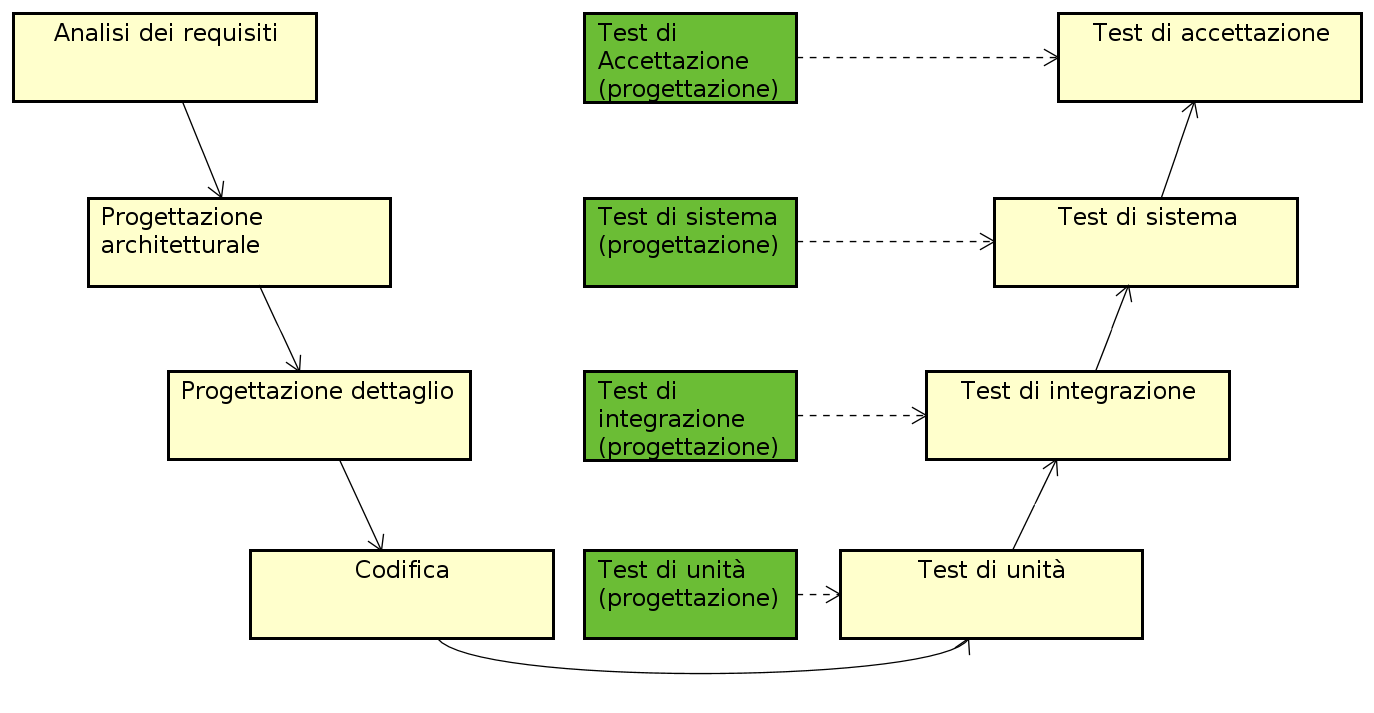
\includegraphics[scale=0.4]{../images/vmodel-final4.png}
%\caption{Fasi di sviluppo}
%\end{figure} 

\newpage
\subsection{Gestione amministrativa della revisione}
Ogni processo coinvolto nell'attività di sviluppo ha bisogno di una costante attività di verifica di supporto in grado di identificare possibili miglioramenti o peggioramenti ed apportare eventuali correzioni. \\
Il modello che il gruppo intende quindi seguire è il cosiddetto PDCA (o Ciclo di Deming), modello volto al miglioramento continuo che definisce quattro fasi cicliche:
\begin{itemize}
\item \textbf{P}lan: definizione del problema, cosa deve essere realizzato e come andrà controllato per la verifica qualitativa;
\item \textbf{D}o: eseguire le attività secondo i piani;
\item \textbf{C}heck: verifica nel tempo dei risultati conseguiti in seguito a modifiche e migliorie, confronto tra risultati attesi e risultati effettivi; %spero di non aver stravolto questo punto, apparte questo il resto va bene
\item \textbf{A}ct: applicazione di soluzioni correttive atte al miglioramento.
\end{itemize}
%(vedere Appendice A per una descrizione dettagliata).\\
Ogni processo deve essere sottoposto a verifica in modo da poterlo migliorare all'iterazione successiva. 
Le due fasi chiave del modello PDCA sono la prima fase di definizione (P) del problema e la fase di verifica dei risultati attesi (C). 
\begin{figure}[h!]
\centering
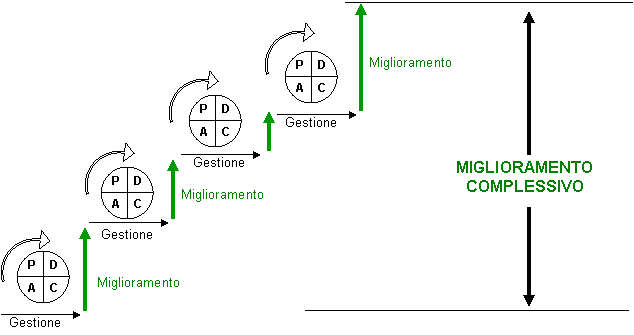
\includegraphics[scale=0.6]{../images/PDCA}
\caption{PDCA e miglioramento complessivo}
\end{figure}
Il concetto generale fa riferimento anche al metodo di \textit{Correctness by construction}, che ha come principio base quello di fare in modo di non introdurre errori già dall'inizio e/o di correggere tali errori nel \textbf{momento più vicino possibile a quando sono stati introdotti}.\\ L'attività costante di verifica, quindi,  deve servire proprio a far sì che gli errori e le divergenze vengano individuate il prima possibile.\\
Piccoli errori iniziali, se non gestiti, possono portare all'assoluta ingestibilità dell'attività di verifica e quindi compromettere pesantemente il successo finale del progetto. Per evitare ciò, un processo dipendente da un altro non può avere inizio finché il precedente non sia stato verificato e ne sia stata accertata la correttezza.\\\\ %ho scambiato due frasi perchè erano abbastanza scollegate prima
Nella sezione Misure e metriche vengono elencate due metriche (\textbf{Schedule variance} e \textbf{Budget variance}) necessarie al controllo e alla valutazione dei processi in termini di tempo (schedule) e in termini di costo e risorse impiegate (budget). 
Tali misurazioni, da effettuare alla fine di ogni fase, si basano sui valori dei consuntivi di ogni fase (presenti nel documento \textit{piano\_di\_progetto\_1.0.pdf}). La valutazione di queste metriche è essenziale per verificare l'andamento di ogni processo misurato e valutarne quindi il miglioramento o il peggioramento complessivo. \\
Per il coordinamento delle attività giornaliere ci si affida ad un sistema di \textbf{ticketing\addglos} fornito dalla piattaforma online \textbf{Trello}\addglos (vedere documento \textit{norme\_di\_progetto\_1.0.pdf} per una spiegazione dettagliata del suo utilizzo). Tale sistema permette di tenere costantemente sotto controllo l'andamento dei compiti (\textbf{Task}\addglos) e la loro realizzazione. 


\subsection{Procedure di controllo di qualità di processo}
Le linee guida fornite dal modell PDCA per l'attività di controllo ed il miglioramento continuo dei processi sono:
\begin{itemize}
\item Pianificazione dettagliata
\item Monitoraggio costante delle attività pianificate in esecuzione
\item Definizione delle risorse umane e tecnologiche necessarie per il conseguimento degli obiettivi
\item Utilizzo di metriche per quantificare e verificare il miglioramento della qualità del processo
\end{itemize}  
Sui processi, quindi, vanno effettuate delle misurazioni oggettive che possano dare informazioni utili sull'andamento degli stessi, in modo da poter decidere se intervenire in maniera migliorativa. 
In generale, tali misurazioni tengono conto dei seguenti elementi: 
\begin{itemize}
\item Tempo impiegato per il completamento
\item Risorse utilizzate 
\item Attinenza alla pianificazione
\end{itemize}
Tramite le piattaforme Trello e GitHub i verificatori possono tenere traccia dello storico dei ticket assegnati, valutarne quindi i tempi di completamento e agire in modo propositivo nel caso si verifichino ritardi nella realizzazione di compiti assegnati.
La verifica del completamento dei ticket viene integrata con un controllo altrettanto costante dell'attività dei commit sulla piattaforma GitHub. Sarà quindi necessario osservare e verificare l'andamento dei commit, verificandone sia correttezza che frequenza.
In periodi di alta attività il numero di commit per persona deve essere maggiore o uguale a 1 (viene inteso un commit significativo relativo all'intera giornata di lavoro) 
%da qui in poi il resto del documento è abbastanza incompleto (quello che c'è però va bene) e ti darò una mano a finirlo in questi giorni
%ti prego però, non scrivere ancora la parola "verifica", usa qualche sinonimo che l'hai ripetuta tipo 40 volte XD
%\subsubsection{Procedure di controllo fi qualità prodotto}
%\begin{itemize}
%\item \textbf{Software Quality Assurance}
%\item \textbf{Verifica}
%\item \textbf{Validazione}
%\end{itemize}
%\section{Risorse per la verifica}

%\subsection{Risorse umane}
%Le risorse attivamente coinvolte nel processo di verifica sono le seguenti: 
%\begin{itemize}
%\item \textbf{Responsabile}: Ha il compito di coordinare le attività di verifica e il controllo di qualità dei processi interni. Distribuisce le risorse sulle attività e ne monitora il corretto svolgimento.
%\item \textbf{Verificatore}: svolge l'effettiva attività di verifica su ogni prodotto. I risultati di tali compiti, che saranno gli esiti delle attività di misurazione, vengono presentati al Responsabile di progetto per la gestione della loro risoluzione.
%\end{itemize}
%Per una più completa ed approfondita descrizione di ogni ruolo si rimanda ai documenti  \textit{Piano-di-progetto-1.0.pdf} e \textit{Norme-di-Progetto.pdf} (sezione 4.2).
%\begin{itemize} 
%\item \textbf{Amministratore}: coordina l’attività di verifica e ne definisce metodologie e norme. Ha l’incarico di gestire la risoluzione di anomalie e discrepanze.
%\item \textbf{Analista}: aggiorna/modifica i requisiti ed i casi d’uso in caso di necessità in seguito a verifica.
%\item \textbf{Progettista}: modifica la struttura dell’architettura di sistema in caso di necessità in seguito a verifica.
%\item \textbf{Programmatore}: durante la fase di programmazione si occupa, oltre alla stesura
%del codice, di attività di debugging per il controllo e/o correzione del codice da lui prodotto. Si occupa anche di applicare le correzioni riscontrate dall’attività di verifica da parte del Verificatore.
%\end{itemize}

%\subsection{Risorse tecnologiche}
%
%Le risorse tecnologiche coinvolte nel processo di verifica sono principalmente le seguenti: 
%\begin{itemize}
%\item \textbf{Complexity-report}: strumento software per l'analisi statica del codice JavaScript;
%\item \textbf{MySpell}: correttore ortografico integrato all'interno di TexMaker;
%\item \textbf{Trello}: piattaforma online per l'organizzazione e la gestione di progetti. 
%\end{itemize}
%\textit{Si rimanda alla sezione Misure e Metriche del presente documento per una spiegazione dettagliata delle metriche utilizzate da Complexity-report, e al documento Norme-di-progetto.pdf per quanto riguarda le modalità di utilizzo dei sopracitati software.} 
\subsection{Procedure di controllo qualità di prodotto}
\begin{itemize}
\item \textbf{Software Quality Assurance}: insieme delle attività volte al fine di garantire il raggiungimento degli obiettivi di qualità. Queste attività prevedono l'utilizzo di tecniche di analisi statica e dinamica
\item \textbf{Verifica}: attività costante durante l'intera fase del progetto; serve a controllare che l'output aspettato dalle entità in oggetto di verifica.
\item \textbf{Validazione}: la conferma oggettiva che il sistema soddisfa i requisiti. 

\end{itemize}
\newpage

\section{Misure e metriche: parametri di tolleranza}
Di seguito vengono elencate le metriche adottate per il controllo qualitativo dei processi, dei documenti e del prodotto software in sviluppo. Per una dettagliata descrizione di ogni metrica vedere la sezione appendici in coda al documento. 
\subsection{Processi}
Metriche utilizzate per il controllo dell'andamento dei processi di supporto allo sviluppo:
\begin{center}
\begin{tabular}{{p{8cm} p{2.5cm} p{2cm}}}
\textbf{Metrica} & \textbf{Accettazione} & \textbf{Ottimale}\\ \hline
Schedule Variance &  \begin{math}\ge -(P*5\%)\end{math} & \begin{math} \ge 0\end{math} \\ \hline
Budget Variance & \begin{math} \ge -(P*10\%) \end{math} & \begin{math} \ge 0 \end{math}\\ \hline
\end{tabular}
\end{center}
\textit{P = PreventivoFase}\\\\
\textit{Schedule variance} e \textit{budget variance} danno un resoconto in termini di tempo e di costi effettuati confrontati con il preventivo.\\
I margini di tolleranza di errore sono stati impostati al 5\% sulle scadenze prefissate e al 10\% sul budget.
\subsection{Documenti}
La metrica che si è scelto di utilizzare per un'analisi il più possibile oggettiva sul contenuto dei documenti è l'indice Gullpease (vedere appendice X per una descrizione più completa). 
\begin{center}
\begin{tabular}{{p{8cm} p{2.5cm} p{2cm}}}
\textbf{Metrica} & \textbf{Accettazione} & \textbf{Ottimale}\\ \hline
Gulpease Index &  \begin{math}[50 - 100]\end{math} & \begin{math}[60 - 100]\end{math} \\ \hline
\end{tabular}
\end{center}
Oltre a questo, la documentazione subisce un processo di verifica più approfondito secondo le seguenti linee guida:  
\begin{itemize}
\item Verifica della presenza di tutti i documenti necessari;
\item Attinenza di ogni documento alle specifiche di stile e formattazione presenti nel documento \textit{Norme-di-progetto-1.0};
\item Verifica della presenza e del corretto utilizzo del registro delle modifiche interno ad ogni documento;
\item Verifica iniziale dei documenti tramite la tecnica di analisi statica \textbf{walkthrough};
\item Verifica dei documenti tramite tecnica di analisi statica di tipo \textbf{inspection}. In questo caso l'attenzione del verificatore si focalizza solo su particolari aspetti del testo (per esempio accenti, sillabazione, maiuscole, ecc);
\item Monitoraggio da parte dei verificatori del registro delle modifiche in modo da poter attuare la verifica solo alla parte inerente alla sezione modificata;
\item \textbf{Coerenza} di informazioni tra i diversi documenti;
\item Verifica di assenza di \textbf{ridondanza} di determinati contenuti tra i diversi documenti;
\item Calcolo dell'indice di leggibilità \textbf{Gulpease}.
\end{itemize}

\subsection{Software}
Per l'analisi statica del codice prodotto viene utilizzato il software di analisi Complexity-report, per una descrizione dettagliata delle metriche utilizzate dal software vedere appendice B sezione 3.5.
\begin{center}
\begin{tabular}{{p{8cm} p{2.5cm} p{2cm}}}
\textbf{Metrica} & \textbf{Accettazione} & \textbf{Ottimale}\\ \hline
Parameters count & \begin{math}[0 - 7]\end{math} & \begin{math}[0 - 5]\end{math}\\ \hline
Dependency count & \begin{math} \le 5 \end{math} &\begin{math} = 0 \end{math}\\ \hline
Halstead's Volume & \begin{math}[20 - 1500]\end{math} & \begin{math}[20 - 1000]\end{math}\\ \hline
Halstead's Difficulty &  \begin{math}[0 - 30]\end{math} & \begin{math}[0 - 15]\end{math}\\ \hline
Cyclomatic complexity & \begin{math}[0 - 15]\end{math} & \begin{math}[0 - 10]\end{math}\\ \hline
First-order density & \begin{math} \le 20\% \end{math} & \begin{math} \le 15\%  \end{math}\\ \hline
Change cost & \begin{math} \le 50\% \end{math} & \begin{math} \le 40\%\end{math}\\ \hline
Core size & \begin{math} \le 30\% \end{math} & \begin{math} \le 25\%\end{math}\\ \hline
Maintainability Index & \begin{math}[20 - 100]\end{math} & \begin{math}[70 - 100]\end{math}\\ \hline
Copertura dei test & \begin{math}[70 - 100]\end{math}& \begin{math}[80 - 100]\end{math}\\ \hline
\end{tabular}
\end{center}
La metrica fondamentale di questo software è il \textbf{Maintainability Index} che offre un valore sul livello di manutenibilità del codice.\\
I valori di tolleranza fissati per tale indice sono:
\begin{itemize}
\item  \begin{math} MI \ge 20: \end{math} alta manutenibilità
\item \begin{math}10 \leq MI \geq 20: \end{math} moderata manutenibilità
\item \begin{math}MI \leq 10: \end{math} bassa manutenibilità
\end{itemize}
\newpage
\appendix
\addappheadtotoc
\setcounter{table}{0}
\renewcommand{\thetable}{A.\arabic{table}}

\newpage
\section{Misure e Metriche}
\label{Appendice A}
\subsection{Di progetto}
\subsubsection{Schedule Variance}
Il valore SV (schedule variance) indica se si è in linea, in anticipo o in ritardo rispetto alla schedulazione delle attività di progetto pianificate nella baseline.\\
Se SV > 0 significa che il progetto sta producendo (ossia rilasciando deliverable) con maggior velocità a quanto pianificato, viceversa se negativo.
Formula:
\begin{center}
\textbf{SV = BCWP – BCWS\\}
\end{center}
Dati:
\begin{itemize}
\item \textbf{BCWP} (Budgeted Cost of Work Performed): Valore delle attività realizzate alla data corrente.
\item \textbf{BCWS} (Budgeted Cost of Work Scheduled): Costo pianificato per realizzare le attività di progetto alla data corrente.
\end{itemize}
\begin{itemize}
	\item Range-accettazione: \begin{math} [ \ge -(PreventivoFase*5\%)]
	\end{math}
	\item Range-ottimale: \begin{math}[ \ge 0]\end{math}
	\end{itemize}
\subsubsection{Budget variance} Indica se alla data corrente si è speso di più o di meno rispetto a quanto previsto a budget alla data corrente.\\
Formula: 
\begin{center}
\textbf{BV = BCWS – ACWP}
\end{center}
Dati:
\begin{itemize}
\item \textbf{ACWP} (Actual Cost of Work Performed): Costo effettivamente sostenuto alla data corrente.
\end{itemize}
Se BV > 0 significa che il progetto sta spendendo il proprio budget con minor velocità di quanto pianificato, viceversa se negativo. Il fatto di spendere più velocemente il budget non ha nulla a che fare con il risparmio che se ne può avere, rappresentato invece da CV.\\\\
Parametri utilizzati: 
\begin{itemize}
	\item Range-accettazione: \begin{math}[ \ge -(PreventivoFase*10\%)]
	\end{math}
	\item Range-ottimale: \begin{math}[ \ge 0]\end{math}
	\end{itemize}
\subsection{Per i documenti}

\subsubsection{Indice Gulpease} Indice di leggibilità di un testo tarato sulla lingua italiana. \\
Questo indice considera due variabili linguistiche: la lunghezza della parola e la lunghezza della frase rispetto al numero delle lettere.
La formula per il suo calcolo è la seguente:\\
\begin{center}
\begin{math}
89 - \frac{(300 * NumeroFrasi) - (10 * NumeroLettere)}{NumeroParole}
\end{math}
\end{center}
I risultati sono compresi tra 0 e 100, dove il valore 100 indica la leggibilità più alta e 0 la leggibilità più bassa.\\
In generale risulta che testi con un indice:
\begin{itemize}
\item inferiore a 80 sono difficili da leggere per chi ha la licenza elementare;
\item inferiore a 60 sono difficili da leggere per chi ha la licenza media;
\item inferiore a 40 sono difficili da leggere per chi ha un diploma superiore.
\end{itemize}
\begin{itemize}
\item Range di accettazione: \begin{math}[50 - 100]\end{math}
\item Range ottimale: \begin{math}[60 - 100]\end{math}
\end{itemize}
\subsection{Per il software}

In questa sezione vengono elencate le metriche utilizzate dal software di analisi Complexity-report come \textbf{Maintainability Index}\addglos, \textbf{Metriche di Halstead}\addglos e \textbf{Complessità Ciclomatica}\addglos) e altri indicatori come la percentuale di \textit{Copertura dei test} e la validazione W3C\addglos dei file HTML\addglos.  
\\
Il software complexity-report offre un resoconto delle misurazioni effettuate sull'intero codice, a livello di file, e a livello di funzione presente in ogni file. 
Di seguito vengono presentate le metriche utilizzate per ogni livello.

%\subsubsection{Logical LOC}
%Numero di righe di codice che rappresentano degli statement\addglos. 
\subsubsection{Parameter count}
Numero di parametri per funzione. Valori bassi sono da preferire.
Parametri utilizzati:
\begin{itemize}
	\item Range di accettazione: \begin{math}[0 - 7]\end{math}
	\item Range ottimale: \begin{math}[0 - 5]\end{math}
	\end{itemize}
\subsubsection{Cyclomatic complexity}
Metrica software usata per indicare la complessità ciclomatica di un programma. Rappresenta una misura quantitativa del numero di cammini linearmente indipendenti che si possono percorrere nel codice sorgente.  
La complessità ciclomatica può essere misurata per funzioni individuali, metodi e classi all'interno di un programma.
\begin{itemize}
	\item Range di accettazione: \begin{math}[0 - 15]\end{math}
	\item Range ottimale: \begin{math}[0 - 10]\end{math}
	\end{itemize}
\subsubsection{Metriche di Halstead} Queste metriche sono state concepite per identificare proprietà misurabili del codice e le relazioni tra di esse. Questi numeri sono staticamente calcolati dal codice sorgente.\\
Dati: 
\begin{itemize}
\item \textit{n}\begin{tiny}{\ped{1}} \end{tiny} = numero di operatori distinti;
\item \textit{n}\begin{tiny}{\ped{2}} \end{tiny} = numero di operandi distinti;
\item \textit{N}\begin{tiny}{\ped{1}} \end{tiny} = numero totale degli operatori;
\item \textit{N}\begin{tiny}{\ped{2}} \end{tiny} = numero totale degli operandi.
\end{itemize}

Da questi numeri si possono calcolare le seguenti misure: 
 
\begin{itemize}
\item Program Vocabulary: \textit{n} = \textit{n}\begin{tiny}{\ped{1}} \end{tiny} + \textit{n}\begin{tiny}{\ped{2}} \end{tiny}
\item Program Lenght: \textit{N} = \textit{N}\begin{tiny}{\ped{1}} \end{tiny} + \textit{N}\begin{tiny}{\ped{2}} \end{tiny}
\item \textbf{Volume}: \textit{V = Nlog\begin{tiny}{\ped{2}} \end{tiny}n}
\begin{itemize}
	\item Range di accettazione: \begin{math}[20 - 1500]\end{math}
	\item Range ottimale: \begin{math}[20 - 1000]\end{math}
	\end{itemize}
%\item Number of Delivered Bugs: \textit{B} = 
%\begin{math}
%\frac{V}{3000}
%\end{math}
%\begin{itemize}
%	\item Range di accettazione: \begin{math}[ = 0 ]\end{math}
%	\item Range ottimale: \begin{math}[ \le 2 ]\end{math}
%	\end{itemize}
\item \textbf{Difficulty}: 
\begin{math}
D = \frac{\textit{n}\begin{tiny}{\ped{1}} \end{tiny}}{2} * \frac{\textit{N}\begin{tiny}{\ped{1}} \end{tiny}}{\textit{n}\begin{tiny}{\ped{2}} \end{tiny}}
\end{math}
\begin{itemize}
	\item Range di accettazione: \begin{math}[0 - 30]\end{math}
	\item Range ottimale: \begin{math}[0 - 15]\end{math}
	\end{itemize}
\item \textbf{Effort}: 
\begin{math}
E = D * V
\end{math}
\begin{itemize}
	\item Range di accettazione: \begin{math}[0 - 400]\end{math}
	\item Range ottimale: \begin{math}[0 - 300]\end{math}
	\end{itemize}
\end{itemize} 
\subsubsection{Dependency count}
Conteggio del numero di chiamate di tipo \textbf{require}\addglos di ogni metodo. Valori bassi sono da preferire.
\subsubsection{Maintainability Index} Rappresenta l'indice principale dei risultati dell'analisi effettuata da Plato sull'intero codice. Compreso tra 0 e 100, questo indice rappresenta la relativa facilità di manutenzione del codice analizzato. Valori alti rappresentano miglior manutenibilità.\\
Questo indice viene calcolato utilizzando la seguente formula: \\
\begin{center}
\begin{math}
MI = MAX\bigg[ 0,100 \frac{171-5.2\ln V - 0,23G - 16,2\ln L}{171} \bigg]
\end{math}
\end{center}
dove: 
\begin{itemize}
\item \textbf{MI} = Maintainability Index
\item \textbf{V} = Halstead Volume
\item \textbf{L} = Source Lines of Code (SLOC)
\item \textbf{G} = Complessità Ciclomatica totale
\end{itemize}
Parametri utilizzati: 
\begin{itemize}
	\item Range di accettazione: \begin{math}[20 - 100]\end{math}
	\item Range ottimale: \begin{math}[70 - 100]\end{math}
	\end{itemize}
%\begin{figure}[h!]
%\centering
%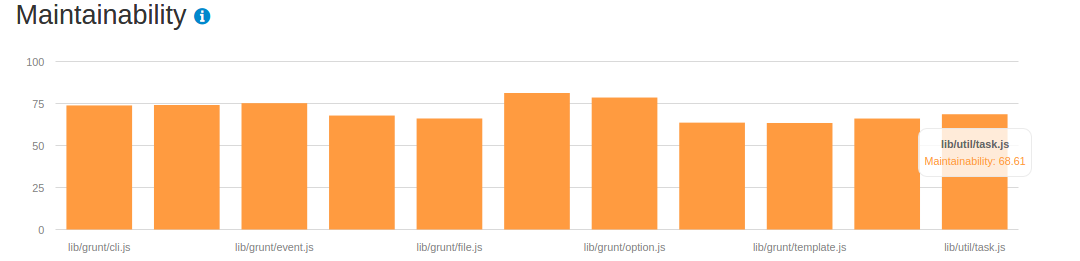
\includegraphics[scale=0.40]{plato_main.png}
%\caption{Plato report - Maintainability Index vista generale}
%\end{figure}
%Oltre alla valutazione generale sull'intero insieme dei file .js, Plato offre una visione specifica per ogni singolo file e per ogni funzione all'interno di un file: 
%\begin{figure}[h!]
%\centering
%\caption{Plato report - file singolo}
%\end{figure}
%I valori mostrati in questa sezione dedicata al singolo file sono i seguenti: 
%\begin{itemize}
%\item \textbf{Maintainability}: (vedere sezione precedente)
%\item \textbf{Lines of Code}: numero di righe del file.
%\item \textbf{Difficulty}: Valore calcolato tramite la funzione di Halstead (vedere sezione 3.4.3.1), rappresenta una misura di quanto il programma può essere difficile da scrivere o da capire.
%\item \textbf{Estimated Errors}: valore che rappresenta una stima del numero di errori di implementazione (Halstead's Number of delivered Bugs).
%\end{itemize}

%\newpage
%\begin{itemize}
%\item \textbf{Source Lines Of Code (SLOC)}: numero di linee del codice sorgente in oggetto. Parametro utilizzato per il calcolo del \textbf{Maintainability Index}.
%\begin{figure}[h!]
%\centering
%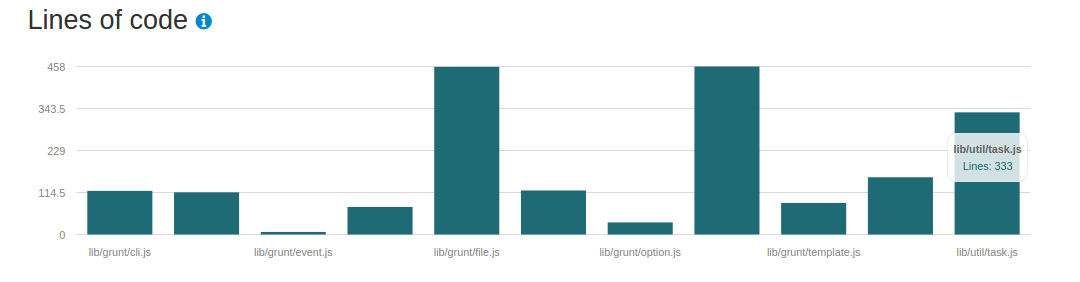
\includegraphics[scale=0.40]{plato_SLOC.png}
%\caption{Plato report - SLOC vista generale}
%\end{figure}
%\item \textbf{Estimated errors in implementation}: stima del numero di errori di implementazione. Valore calcolato tramite la metrica di \textit{Halstead}.

%\begin{figure}[h!]
%\centering
%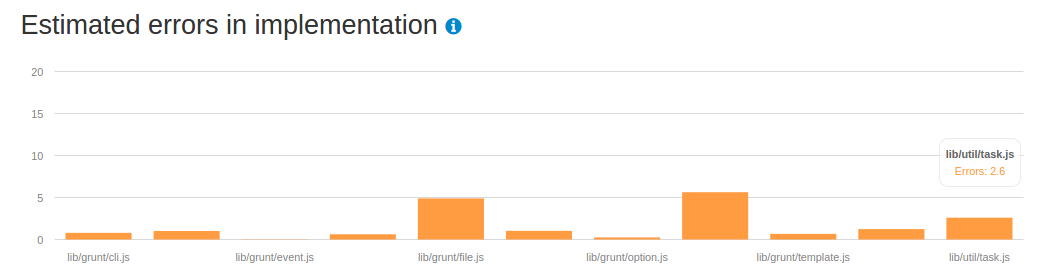
\includegraphics[scale=0.40]{plato_est.png}
%\caption{Plato report - Estimated errors in implementation}
%\end{figure}

%\item \textbf{Lint errors}: DESCRIZIONE
%\begin{figure}[h!]
%\centering
%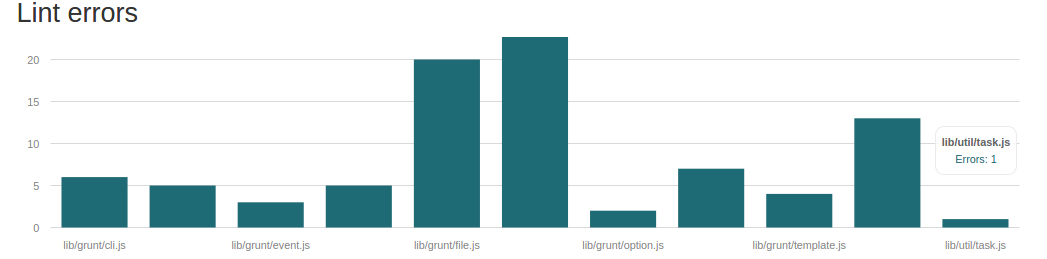
\includegraphics[scale=0.40]{plato_lint.png}
%\caption{Plato report - Lint errors}
%\end{figure}
%\end{itemize}
\subsubsection{First-order density}
Percentuale di tutte le possibili dipendenze interne tra i moduli del progetto. 
\begin{itemize}
	\item Range di accettazione: \begin{math}[\le 20\%]\end{math}
	\item Range ottimale: \begin{math}[\le 15\%]\end{math}
	\end{itemize}
\subsubsection{Change cost}
Percentuale dei moduli affetti da cambiamento quando un modulo all'interno del progetto viene modificato.
\begin{itemize}
	\item Range di accettazione: \begin{math}[\le 50\%]\end{math}
	\item Range ottimale: \begin{math}[\le 40\%]\end{math}
	\end{itemize}
\subsubsection{Core size}
La percentuale dei moduli che hanno molte dipendenze verso (e da) altri moduli.
\begin{itemize}
	\item Range di accettazione: \begin{math}[\le 30\%]\end{math}
	\item Range ottimale: \begin{math}[\le 25\%]\end{math}
	\end{itemize}
\subsubsection{Copertura dei test}
Indica la percentuale dei casi testati rispetto alla totalità dei casi da testare. Una percentuale del 100\% può essere auspicabile solo se sono stati ben definiti i casi che necessitano realmente di essere testati. 
\begin{center}
\textit{Copertura dei test = Numero funzioni testate * 100/Numero funzioni da testare}
\end{center}
Parametri utilizzati: 
\begin{itemize}
	\item Range-accettazione: \begin{math}[70 - 100]\end{math}
\item Range-ottimale: \begin{math}[80 - 100]\end{math}
	\end{itemize}
\subsubsection{W3C - Markup Validation Service}
Per la validazione delle pagine HTML e i file CSS sviluppati si intende affidarsi allo strumento online W3C Markup Validation Service (\url{https://validator.w3.org/}). 

%\subsubsection{Use Case Points}
%non so se metterla o meno
%\begin{itemize}
%\item \textbf{Nodejs}:
%\item \textbf{Complessità ciclomatica}:
%\item \textbf{Numero metodi}:
%\item \textbf{Variabili non utilizzate o non definite}:
%\item \textbf{Numero parametri per metodo}:
%\item \textbf{Numero di livelli di annidamento}
%\item \textbf{Grado di accoppiamento}:
%\item \textbf{Copertura del codice}:
%\item \textbf{Use Case points}:
%\item \textbf{Statement Coverage}:
%\item \textbf{Branch Coverage}:
%\item \textbf{Validazione W3C}:
%\end{itemize}
%\newpage

\newpage
\section{Specifica test}
\label{Appendice B} 
La suddivisione temporale delle diverse fasi di sviluppo segue il cosiddetto modello a V ed è descritta nel documento allegato \textit{Piano-di-Progetto-1.0.pdf}.
\begin{figure}[h!]
\centering
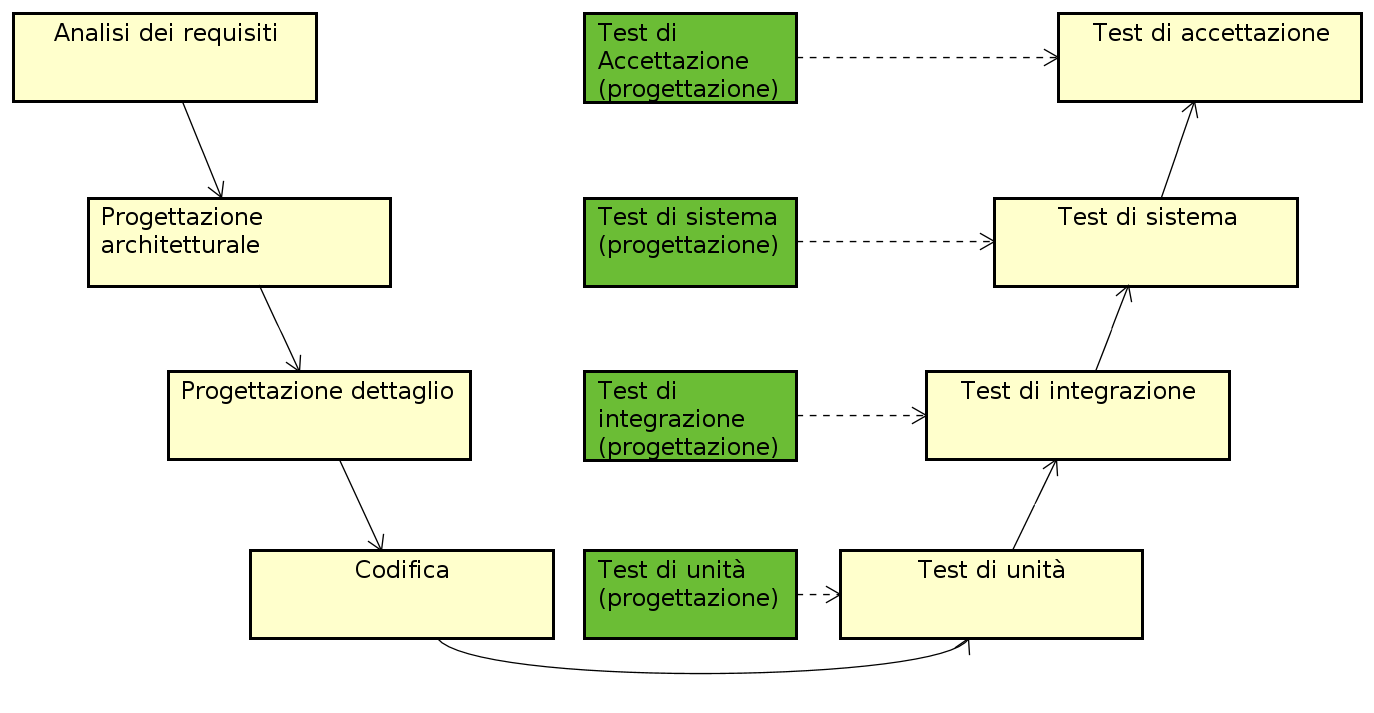
\includegraphics[scale=0.4]{../images/vmodel-final4.png}
\caption{Fasi di sviluppo}
\end{figure} 
%questo paragrafo era abbastanza da rivedere, ora credo sia più chiaro ma aspetto anche la revisione di andrea e casomai lo modificheremo ancora
Questo modello prevede un lavoro di controllo e verifica corrispondente ad ogni attività per evitare l'accumulo di errori difficilmente gestibili in seguito.\\
La divisione in diverse fasi, e l'attività di verifica abbinata ad ogni fase e processo, hanno come scopo quello di facilitare l'integrazione e il corretto funzionamento delle parti che comporranno il sistema finale.
Il ramo discendente descritto nella precedente figura rappresenta la successione delle fasi di sviluppo: ciascuna fase è accompagnata da una costante attività di verifica in modo da poter permettere il passaggio alla fase successiva esclusivamente quando si è sicuri che non ci siano errori. Ciò è essenziale durante la delicata attività di raccolta e documentazione dei requisiti, nella progettazione architetturale ad alto livello ed in seguito nella progettazione di dettaglio.\\ 
%in questa frase non capivo proprio cosa volevi dire, nel dubbio sotto la mia frase ti lascio quello che avevi scritto se vuoi rimetterlo
Del ramo ascendente che attraversa le attività di testing è importante sottolineare l'utilizzo dell'approccio bottom-up.
%Per quanto riguarda il ramo ascendente, da notare l'essenziale importanza, per l'attività di testing,  dell'approccio bottom-up che inizia nel ramo più basso del diagramma. 
Dalla fase di codifica quindi, per mezzo di test specifici sulle singole componenti (test di unità), si è in grado di garantire la correttezza del lavoro svolto prima che le singole componenti vengano integrate tra loro. Ovviamente l'esito positivo di ogni test su ogni unità non garantisce la correttezza dell'integrazione tra le stesse. \\
\subsection{Livelli di testing}
I test da pianificare ed effettuare, come spiegato nel documento \textit{Norme-di-progetto-2.0.pdf}, sono divisi in quattro categorie:
\begin{itemize}
\item \textbf{Test di Accettazione (TA)}
\item \textbf{Test di Sistema (TS)}
\item \textbf{Test di Integrazione (TI)}
\item \textbf{Test di Unità (TU)}
\end{itemize}
\subsection{Test di accettazione}
	\subsubsection{Requisiti funzionali}
			\begin{longtable}{p{0.15\columnwidth}p{0.15\textwidth}p{0.5\columnwidth}p{0.2\textwidth}}
			\caption{Test di accettazione} \\

\textbf{ID requisito} & \textbf{ID test} & \textbf{Descrizione} & \textbf{Stato} \\
\midrule
\endfirsthead

ID & Descrizione & Stato \\
\midrule
\endhead

\multicolumn{2}{c}{\footnotesize\itshape\tablename~\thetable: Requisiti funzionali}
\endfoot

\multicolumn{2}{c}{\footnotesize\itshape\tablename~\thetable: Requisiti funzionali}
\endlastfoot
F 1 \newline F 1.1 \newline F 1.1.1 \newline F 1.1.2 \newline F1.1.2.1&TA 1&Viene verificato che il sistema fornisca la possibilità ad un utente non autenticato di registrarsi compilando il form di registrazione.
L'utente deve poter: 
\begin{enumerate}
\item inserire la propria mail
\item inserire la password
\item ricevere un messaggio di errore se la stringa password ha meno di 8 caratteri
\item inviare i dati di registrazione
\end{enumerate} & Pianificato\\
\midrule
%F 1.1 &TA 1.1& La sezione dedicata alla registrazione deve permettere l'inserimento dei dati necessari & Pianificato\\
%\midrule
%F 1.1.1 &TA 1.1.1& La sezione dedicata alla registrazione deve permettere l'inserimento di una e-mail & Pianificato\\
%\midrule
%F 1.1.2 &TA 1.1.2& La sezione dedicata alla registrazione deve permettere l'inserimento di una password & Pianificato\\
%\midrule
%F 1.1.2.1 &TA 1.1.2.1& Se la password inserita ha meno di 8 caratteri viene visualizzato un messaggio di errore & Pianificato\\
%\midrule
F 1.2 \newline F 1.2.1 \newline F 1.2.1.1 \newline F 1.2.1.2 \newline F 1.2.1.3 & TA 1.2&La sezione dedicata alla registrazione deve permettere l'invio dei dati inseriti. L'utente deve poter ricevere un messaggio di errore se: 
\begin{enumerate}
\item i dati non sono stati inseriti
\item la mail inserita risulta già in uso
\end{enumerate}
Se i dati non sono corretti il sistema deve bloccare l'invio. & Pianificato\\
%\midrule
%F 1.2.1 &TA 1.2.1&Prima di inviare i dati viene effettuato un controllo su di essi & Pianificato\\
%\midrule
%F 1.2.1.1 & TA 1.2.1.1&Se i dati richiesti non sono stati inseriti viene visualizzato un messaggio di errore & Pianificato\\
%\midrule
%F 1.2.1.2 &TA 1.2.1.2&Se la email inserita risulta già in uso viene visualizzato un messaggio di errore & Pianificato\\
\midrule
%F 1.2.1.3 & TA 1.2.1.3&Se i dati non risultano corretti ne viene bloccato l'invio & Pianificato\\

F 1.2.2 \newline F 1.2.3 & TA 1.2.2 & Quando i dati corretti vengono inviati viene verificato che:
\begin{enumerate}
\item il sistema memorizzi un nuovo account con i dati inseriti
\item venga effettuato automaticamente il login al completamento della registrazione
\end{enumerate}   & Pianificato\\

%F 1.2.3 & TA 1.2.3&Quando viene creato un nuovo account con la procedura di registrazione viene automaticamente effettuato il login con quell'account & Pianificato\\
\midrule
F 2 \newline F 2.1 \newline F 2.1.1 \newline F2.1.2  & TA 2& Verifica che il sistema fornisca la possibilità ad un utente non autenticato di autenticarsi. All'utente dev'essere permesso di: 
\begin{enumerate}
\item inserire la propria mail
\item inserire la propria password
%\item recuperare la propria password se dimenticata
\item
\end{enumerate} & Pianificato\\

%F 2.1 &TA 2.1 & La sezione dedicata all'autenticazione deve permettere l'inserimento dei dati necessari & Pianificato\\
%\midrule
%F 2.1.1 &TA 2.1.1&La sezione dedicata all'autenticazione deve permettere l'inserimento di una e-mail & Pianificato\\
%\midrule
%F 2.1.2 &TA 2.1.2&La sezione dedicata all'autenticazione deve permettere l'inserimento di una password & Pianificato\\
%\midrule
F 2.2 \newline F 2.2.1 \newline F 2.2.2 \newline F 2.2.2.1 \newline F 2.2.2.2 \newline F 2.2.3&TA 2.2&Verifica che la sezione dedicata all'autenticazione fornisca una procedura di recupero password. il sistema deve:
\begin{enumerate}
\item permettere l'nserimento della mail
\item controllare che la mail risulti registrata e in caso negativo visualizzare un messaggio di errore
\item bloccare l'invio dei dati se la mail non risulta registrata
\item mandare una mail all'indirizzo inserito con la password dimenticata
\end{enumerate} & Pianificato\\
\midrule
%F 2.2.1 &TA 2.2.1&La procedura di recupero password deve permettere l'inserimento della e-mail & Pianificato\\
%\midrule
%F 2.2.2 &TA 2.2.2&La procedura di recupero password deve effettuare un controllo sulla e-mail inserita & Pianificato\\
%\midrule
%F 2.2.2.1 &TA 2.2.2.1&Se la e-mail non risulta registrata viene visualizzato un messaggio di errore & Pianificato\\
%\midrule
%F 2.2.2.2 & TA 2.2.2.2&Se la e-mail non risulta registrata viene bloccato l'invio della mail a quell'indirizzo & Pianificato\\
%\midrule
%F 2.2.3 & TA 2.2.3&La procedura di recupero password deve mandare una mail all'indirizzo inserito con la password dimenticata & Pianificato\\
%\midrule
F 2.3 \newline F 2.3.1 \newline F 2.3.1.1 \newline F 2.3.2 & TA 2.3& Verifica che la sezione dedicata all'autenticazione permetta l'invio dei dati inseriti. Il sistema deve: 
\begin{enumerate}
\item effettuare un controllo di correttezza sui dati inseriti
\item visualizzare un messaggio di errore se la combinazione e-mail/password non è registrata
\item autenticare l'utente se la combinazione mail/password è corretta
\end{enumerate} & Pianificato\\
\midrule
%F 2.3.1 & TA 2.3.1&Prima di inviare i dati viene effettuato un controllo su di essi & Pianificato\\
%\midrule
%F 2.3.1.1 & TA 2.3.1.1 &Se la combinazione e-mail/password non è registrata viene visualizzato un messaggio di errore & Pianificato\\
%\midrule
%F 2.3.2 & TA 2.3.2 &Se la combinazione e-mail/password è registrata l'utente viene autenticato & Pianificato\\
%\midrule
F 3 \newline F 3.1 \newline  F 3.1.1 \newline  F 3.1.2 \newline F 3.1.3& TA 3 &Verifica che il sistema permetta la navigazione e selezione dei questionari per categoria. Il sistema deve: 
\begin{enumerate}
\item fornire una sezione con un elenco di categorie
\item fornire l'elenco dei questionari presenti per la categoria selezionata
\item fornire il numero di questionari della categoria
\end{enumerate} & Pianificato\\
\midrule
%F 3.1 & TA 3.1 &Il sistema deve fornire una sezione con un elenco delle categorie di questionari presenti nel database & Pianificato\\
%\midrule
%F 3.1.1 & TA 3.1.1 &Quando l'utente seleziona una categoria viene visualizzata la sezione che elenca i questionari della categoria scelta & Pianificato\\
%\midrule
%F 3.1.2 & TA 3.1.2 &Per ogni elemento dell'elenco viene visualizzato il nome della categoria & Pianificato\\
%\midrule
%F 3.1.3 & TA 3.1.3 &Per ogni elemento dell'elenco viene visualizzato il numero di questionari della categoria & Pianificato\\
%\midrule
F 3.2 \newline F 3.2.1 \newline  F 3.2.2 \newline  F 3.2.3 \newline F 3.2.4& TA 3.2 &Verifica che il sistema fornisca una sezione con un elenco dei questionari relativi ad una categoria. Viene verificato che: 
\begin{enumerate}
\item uando l'utente seleziona un questionario venga visualizzata la sezione della compilazione del questionario scelto
\item per ogni elemento dell'elenco venga visualizzato il nome del questionario
\item per ogni elemento dell'elenco venga visualizzato il numero di domande del questionario
\item per ogni elemento dell'elenco venga visualizzato l'autore
\end{enumerate} & Pianificato\\
%\midrule
%F 3.2.1 &TA 3.2.1&Quando l'utente seleziona un questionario viene visualizzata la sezione della compilazione del questionario scelto & Pianificato\\
%\midrule
%F 3.2.2 &TA 3.2.2&Per ogni elemento dell'elenco viene visualizzato il nome del questionario & Pianificato\\
%\midrule
%F 3.2.3 & TA 3.2.3 &Per ogni elemento dell'elenco viene visualizzato il numero di domande del questionario & Pianificato\\
%\midrule
%F 3.2.4 &TA 3.2.4 &Per ogni elemento dell'elenco viene visualizzato l'autore & Pianificato\\
\midrule
F 4 \newline F 4.1 \newline F 4.2 \newline F 4.2.1 \newline F 4.2.2 \newline F 4.2.3 \newline F 4.2.4 \newline F 4.2.4.1 \newline F 4.2.5 \newline F 4.2.5.1 \newline F 4.2.6 \newline F 4.2.6.1 \newline F 4.3 \newline F 4.4& TA 4& Verifica che il sistema dia la possibilità di compilare un questionario.\newline L'utente deve poter:
\begin{enumerate}
\item navigare liberamente tra le domande del questionario
\item rispondere alle domande
\item visualizzare la risposta data
\item selezionare possibili risposte in caso di risposte multiple
\item associare elementi in caso di risposte di tipo associativo
\item selezionare le risposte in caso di domanda di tipo completamento testo
\item cambiare le risposte già date
\item rispondere alle domande in qualsiasi ordine
\item consegnare il questionario completato

\end{enumerate} & Pianificato\\

%F 4.1 &TA 4.1 &Durante la compilazione del questionario un utente può navigare liberamente tra le domande che lo compongono & Pianificato\\
%\midrule
%F 4.2 & TA 4.2 &L'utente può rispondere alle domande & Pianificato\\
%\midrule
%F 4.2.1 &TA 4.2.1&Viene visualizzato il testo della domanda & Pianificato\\
%\midrule
%F 4.2.2 &TA 4.2.2 &Viene visualizzata la risposta data & Pianificato\\
%\midrule
%F 4.2.3 & TA 4.2.3 &Se la domanda richiede una risposta inserita dal'utente allora viene fornito un campo per l'inserimento della risposta & Pianificato\\
%\midrule
%F 4.2.4 &TA 4.2.4 &Se la domanda ha delle risposte preimpostate di qualsiasi tipo queste vengono visualizzate & Pianificato\\
%\midrule
%F 4.2.4.1 & TA 4.2.4.1 &Deve essere possibile selezionare una risposta & Pianificato\\
%\midrule
%F 4.2.5 & TA 4.2.5 &Se la domanda permette associazioni tra elementi deve visualizzare tutti gli elementi associabili & Pianificato\\
%\midrule
%F 4.2.5.1 & TA 4.2.5.1 &Deve essere possibile associare due elementi di insiemi diversi & Pianificato\\
%\midrule
%F 4.2.6 & TA 4.2.6 &Se la domanda prevede il completamento del testo con delle parole vengono visualizzate le possibili parole & Pianificato\\
%\midrule
%F 4.2.6.1 & TA 4.2.6.1 &Deve essere possibile selezionare una parola dalla lista & Pianificato\\
%\midrule
%F 4.3 & TA 4.3&L'utente può cambiare la risposta di una domanda in qualsiasi momento prima della consegna del questionario & Pianificato\\
%\midrule
%F 4.4 & TA 4.4 &Le domande possono essere compilate in un ordine qualsiasi & Pianificato\\
%\midrule
%F 4.5 &TA 4.5 &L'utente può consegnare il questionario & Pianificato\\
\midrule
F 4.5.1 \newline F 4.5.2 \newline F 4.5.2.1 \newline F 4.5.2.1.1 \newline F 4.5.2.1.2 \newline F 4.5.2.1.3& TA 4.5.1 &Verifica che alla consegna del questionario il sistema: 
\begin{enumerate}
\item avvisi l'utente se alcune risposte non sono state compilate
\item valuti il questionario e ne visualizzi il risultato
\item visualizzi il punteggio ottenuto
\item visualizzi la percentuale di risposte corrette 
\end{enumerate} & Pianificato\\
\midrule
%F 4.5.2 & TA 4.5.2 &Quando un questionario viene confermato e consegnato viene valutato dal sistema & Pianificato\\
%\midrule
%F 4.5.2.1 & TA 4.5.2.1 &La valutazione del questionario viene visualizzata all'utente & Pianificato\\
%\midrule
%F 4.5.2.1.1 &TA 4.5.2.1.1 &Viene visualizzato il nome del questionario & Pianificato\\
%\midrule
%F 4.5.2.1.2 & TA 4.5.2.1.2 &Viene visualizzato il punteggio ottenuto & Pianificato\\
%\midrule
%F 4.5.2.1.3 & TA 4.5.2.1.3 &Viene visualizzata la percentuale delle risposte corrette & Pianificato\\
%\midrule

F 4.6 \newline F 4.6.1 \newline F 4.6.2 \newline F 4.7& TA 4.6&Verifica che la compilazione del questionario abbia un tempo massimo. \newline
Il sistema deve:
\begin{enumerate}
\item consegnare automaticamente il questionario allo scadere del tempo massimo anche se incompleto
\item visualizzare il tempo restante

\end{enumerate} & Pianificato\\
\midrule
%F 4.6.1 & TA 4.6.1 &Allo scadere del tempo il questionario verrà consegnato automaticamente anche se incompleto & Pianificato\\
%\midrule
%F 4.6.2 & TA 4.6.2 &Il tempo inizia a scorrere da quando l'utente accede alla pagina & Pianificato\\
%\midrule
%F 4.7 &TA 4.7 &Viene visualizzato il tempo restante & Pianificato\\
%\midrule
F 5 \newline F 5.1 \newline F 5.1.1 \newline F 5.1.2 \newline F 5.2& TA 5&Verifica che il sistema dia la possibilità ad un utente autenticato di creare una nuova domanda. \newline
L'utente deve potere:
\begin{enumerate}
\item scegliere la categoria della domanda
\item inserire i dati necessari alla compilazione della domanda in formato QML
\item inviare i dati inseriti 
\end{enumerate} & Pianificato\\
\midrule
%F 5.1 &TA 5.1&La sezione dedicata alla creazione di una domanda deve permettere l'inserimento dei dati necessari & Pianificato\\
%\midrule
%F 5.1.1 & TA 5.1.1 &La sezione dedicata alla creazione di una domanda deve permettere la scelta di una o più categorie & Pianificato\\
%\midrule
%F 5.1.2 & TA 5.1.2 &La sezione dedicata alla creazione di una domanda deve permettere l'inserimento del codice QML che definisce la domanda & Pianificato\\
%\midrule
%F 5.2 & TA 5.2&La sezione dedicata alla creazione di una domanda deve permettere l'invio dei dati inseriti & Pianificato\\
%\midrule
F 5.2.1 \newline F 5.2.1.1 \newline F 5.2.1.2 \newline F 5.2.1.3 \newline F 5.2.2 \newline F 5.2.2.1 \newline F 5.2.2.2 \newline & TA 5.2.1&Verifica che il sistema effettui un controllo sulla correttezza dei dati prima della memorizzazione. Il sistema deve: 
\begin{enumerate}
\item visualizzare un messaggio di errore se i dati obbligatori non risultano inseriti
\item visualizzare un messaggio di errore se il codice QML inserito non risulta valido
\item visualizzare un messaggio nel caso che i dati siano corretti e la memorizzazione della domanda è andata a buon fine. In caso contrario deve annullare la creazione della domanda ed avvisare l'utente tramite un messaggio a schermo
\end{enumerate} & Pianificato\\
\midrule
%F 5.2.1.1 & TA 5.2.1.1 &Se i dati obbligatori non risultano inseriti viene visualizzato un messaggio di errore & Pianificato\\
%\midrule
%F 5.2.1.2 & TA 5.2.1.2 &Se il codice QML inserito non risulta valido viene visualizzato un messaggio di errore & Pianificato\\
%\midrule
%F 5.2.1.3 &TA 5.2.1.3 &Se i dati obbligatori non risultano inseriti o il codice QML non è valido la creazione della nuova domanda viene bloccata & Pianificato\\
%\midrule
%F 5.2.2 & TA 5.2.2 &Quando dei dati che superano i controlli vengono inviati viene creata una nuova domanda con essi e inserita nel database & Pianificato\\
%\midrule
%F 5.2.2.1 & TA 5.2.2.1 &Se la creazione di una nuova domanda va a buon fine il sistema avvisa l'utente & Pianificato\\
%\midrule
%F 5.2.2.2 & TA 5.2.2.2 & Se la creazione di una nuova domanda non va a buon fine il sistema visualizza un messaggio di errore & Pianificato\\
%\midrule
F 6 \newline F 6.1 \newline F 6.1.1 \newline F 6.1.2 \newline F 6.1.3 \newline F 6.1.3.1 \newline F 6.1.3.2 \newline F 6.2& TA 6& Verifica che il sistema fornisca la possibilità ad un utente autenticato di creare un nuovo questionario. \newline L'utente deve poter: 
\begin{enumerate}
\item compilare il nome del questionario
\item inserire la categoria
\item visualizzare la lista delle domande della categoria
\item selezionare qualsiasi domanda visualizzata
\item inviare il nuovo questinario
\end{enumerate} & Pianificato\\
%\midrule
%F 6.1 &TA 6.1&La sezione dedicata alla creazione di un questionario deve permettere l'inserimento dei dati necessari & Pianificato\\
%\midrule
%F 6.1.1 & TA 6.1.1&La sezione dedicata alla creazione di un questionario deve permettere l'inserimento del nome del questionario & Pianificato\\
%\midrule
%F 6.1.2 &TA 6.1.2 &La sezione dedicata alla creazione di un questionario deve permettere l'inserimento della categoria del questionario & Pianificato\\
%\midrule
%F 6.1.3 &TA 6.1.3 &La sezione dedicata alla creazione di un questionario deve visualizzare la lista delle domande della categoria selezionata & Pianificato\\
%\midrule
%F 6.1.3.1 &TA 6.1.3.1 &Se nessuna categoria è stata selezionata non viene visualizzata alcuna domanda & Pianificato\\
%\midrule
%F 6.1.3.2 & TA 6.1.3.2 &Ogni domanda deve essere selezionabile & Pianificato\\
%\midrule
%F 6.2 & TA 6.2 &La sezione dedicata alla creazione di un nuovo questionario deve permettere l'invio dei dati inseriti & Pianificato\\
\midrule
F 6.2.1 \newline F 6.2.1.1 \newline F 6.2.1.2 \newline F 6.2.1.3 \newline F 6.2.2 \newline F 6.2.2.1 \newline F 6.2.2.2 &  TA 6.2.1 &Verifica che il sistema, prima di inviare i dati, effettui un controllo su di essi. Nello specifico si verifica che il sistema: 
\begin{enumerate}
\item avvisi con un messaggio che i campi obbligatori non sono stati compilati o non è stata selezionata nessuna domanda
\item crei il nuovo questinario se i dati inseriti sono corretti, avvisando l'utente del successo
\item avvisi l'utente con un messaggio se la creazione del nuovo questionario non è andata a buon fine

\end{enumerate} & Pianificato\\
%\midrule
%F 6.2.1.1 & TA 6.2.1.1 &Se i dati obbligatori non risultano inseriti viene visualizzato un messaggio di errore & Pianificato\\
%\midrule
%F 6.2.1.2 &TA 6.2.1.2 &Se nessuna domanda è selezionata viene visualizzato un messaggio di errore & Pianificato\\
%\midrule
%F 6.2.1.3 & TA 6.2.1.3 &Se i dati obbligatori non risultano inseriti non è valido nessun dato viene inviato & Pianificato\\
%\midrule
%F 6.2.2 &TA 6.2.2 &Quando dei dati che superano i controlli vengono inviati viene creato un nuovo questionario con essi e inserito nel database & Pianificato\\
%\midrule
%F 6.2.2.1 &TA 6.2.2.1 &Se la creazione di un nuovo questionario va a buon fine il sistema avvisa l'utente & Pianificato\\
%\midrule
%F 6.2.2.2 & TA 6.2.2.2 &Se la creazione di un nuovo questionario non va a buon fine il sistema visualizza un messaggio di errore & Pianificato\\
%\midrule
%F 7 & TA 7&Il sistema deve fornire la possibilità ad un utente autenticato di uscire facendo il logout & Pianificato\\
%\midrule
%F 8 & TA 8&Il sistema deve essere in grado di interpretare il codice QML & Pianificato\\
%\midrule
%F 8.1 & TA 8.1&QML definisce domande & Pianificato\\
%\midrule
%F 8.1.1 &TA 8.1.1&Una domanda è formata dal testo del quesito e da una o più risposte & Pianificato\\
%\midrule
%F 8.1.2 &TA 8.1.2&Una domanda deve avere almeno una risposta esatta & Pianificato\\
%\midrule
%F 8.1.3 & TA 8.1.3&Una domanda può avere una lista di possibili risposte & Pianificato\\
%\midrule
%F 8.1.4 & TA 8.1.4 &QML permette la definizione di diverse tipologie di domande & Pianificato\\
%\midrule
%F 8.1.4.1 &TA 8.1.4.1 &QML definisce domande di tipo vero o falso & Pianificato\\
%\midrule
%F 8.1.4.2 & TA&QML definisce domande a scelta multipla con una sola risposta esatta & Pianificato\\
%\midrule
%F 8.1.4.3 & TA 8.1.4.3 &QML definisce domande a scelta multipla con più risposte esatte & Pianificato\\
%\midrule
%F 8.1.4.4 & TA 8.1.4.4 &QML definisce domande a risposta testuale & Pianificato\\
%\midrule
%F 8.1.4.5 & TA 8.1.4.5 &QML definisce domande di associazione tra elementi di due insiemi & Pianificato\\
%\midrule
%F 8.1.4.5.1 &TA 8.1.4.5.1 &Gli insiemi possono contenere elementi non associabili di disturbo & Pianificato\\
%\midrule
%F 8.1.4.6 & TA 8.1.4.6&QML definisce domande a completamento testuale a scelta da un gruppo di parole date & Pianificato\\
%\midrule
%F 8.1.4.6.1 & TA 8.1.4.6.1 &Il gruppo di parole può contenere elementi di disturbo & Pianificato\\
%\midrule
%F 8.1.4.7 & TA 8.1.4.7&QML definisce domande di associazione tra date poste in una timeline e avvenimenti & Pianificato\\
%\midrule
%F 8.2 &TA 8.2 &QML gestisce immagini all'interno di domande e risposte preimpostate & Pianificato\\
			
\end{longtable}
\section{Resoconto attività di verifica}
\label{Appendice C}
Di seguito viene fornito il resoconto dell'attività di verifica inerente ad ogni fase di sviluppo.
\end{document}